


The development of an effective visualization framework for explanations, shaped in the form of a synthetic neighborhood and a decision tree surrogate model, requires a departure from traditional textual representation approaches. As established in Subsection \ref{subsec:currentLOREapproach}, current textual formats, as the $\text{LORE}_{sa}$'s one, present critical limitations: significant cognitive load for parsing logical conditions, limited contextual understanding of decision boundaries, static information delivery, and scalability challenges for high-dimensional datasets.

Our approach recognizes that 
% $\text{LORE}_{sa}$ generates two
the two explanation components are 
distinct but complementary information artifacts requiring different visualization paradigms: a \textbf{synthetic neighborhood} in need of spatial representation, and a \textbf{surrogate decision tree} requiring hierarchical visualization of logical structures. 

% %%%%%%%%%%%%%%%%%%%%%%%%
% The limitations identified in Subsection \ref{subsec:currentLOREapproach} reveal fundamental challenges in communicating $\text{LORE}_{sa}$ explanations through textual formats alone: cognitive overload from parsing logical conditions, limited contextual understanding of decision boundaries, invisible neighborhood characteristics, static information delivery, and scalability issues with complex datasets. These challenges are not unique to $\text{LORE}_{sa}$ but reflect broader issues in eXplainable AI systems where rich, multi-dimensional information cannot effectively be communicated through compressed linear text.

% Our visualization framework addresses these limitations using a dual-representation strategy that exploits the distinct nature of $\text{LORE}_{sa}$'s information artifacts. Rather than forcing users to mentally reconstruct spatial relationships from textual descriptions, we provide direct visual access to the synthetic neighborhood through scatter plot visualizations. This spatial representation immediately reveals neighborhood density, distribution patterns, and the position of the explained instance relative to decision boundaries—information that would remain opaque in textual formats. Similarly, instead of requiring users to understand nested logical conditions as text, we employ interactive decision tree visualizations that make hierarchical rule structures directly navigable and explorable.

% The framework's interactive design transforms explanation consumption from passive reading into active investigation. Bidirectional linking between spatial and symbolic representations enables users to confirm the quality of the explanation by directly observing how the rules boundaries correspond to synthetic instance distributions, addressing the contextual understanding gap inherent in static textual presentations. Users can click on points in the scatter plot to trace their classification paths through the decision tree, or select tree nodes to visualize the spatial distribution of instances satisfying specific logical conditions. These interactions reduce cognitive load by externalizing mental integration tasks, allowing the visual system to perform pattern recognition that would be computationally expensive for conscious reasoning.

% Our approach builds on three established principles from visualization and human-computer interaction research. First, \textbf{interactive confirmation supports explanation trust}: bidirectional interaction between neighborhood visualization and rule exploration enables users to validate explanation quality by examining correspondence between rules boundaries and synthetic instance distributions. Second, \textbf{information integration reduces cognitive load}: coordinated views presenting spatial and symbolic information allow users to directly observe relationships between neighborhood characteristics and rule structure without mental integration across separate interfaces. Third, \textbf{multiple representation formats support diverse user mental models}: different visualization formats for the same decision tree structure accommodate diverse cognitive approaches to understanding machine learning explanations.

% The scalability challenges posed by high-dimensional datasets are addressed through dimensionality reduction techniques (UMAP, PCA, t-SNE, MDS) that project complex feature spaces into interpretable two-dimensional visualizations while preserving essential rules boundary characteristics. Unlike textual representations that become increasingly unwieldy as feature dimensionality grows, our visual approach maintains constant interface complexity regardless of the original feature space dimensions. The scatter plot consistently presents a two-dimensional view, while the decision tree visualization scales based on surrogate model complexity rather than input dimensionality.

% The framework structures the explanation workflow around three sequential but iterative phases: \textbf{Understanding} synthetic neighborhood quality through scatter plot exploration; \textbf{Exploring} the surrogate model structure through interactive decision tree navigation; and \textbf{Confirming} extracted rules through cross-referencing between spatial and symbolic representations. This workflow reflects the natural progression of explanation comprehension while supporting iterative refinement as users develop a deeper understanding.

% Our implementation focuses on coordinating spatial neighborhood analysis with the interactive surrogate model interface, as illustrated in Figure \ref{fig:dual_representation_overview}. The following subsections detail the conceptual framework underlying this integration and describe the interactive confirmation model that transforms passive explanation consumption into active analytical investigation.

% %%%%%%%%%%%%%%%%%%%%%%%%

\subsection{Conceptual Framework}

Our framework addresses this fundamental disconnect through an \textbf{integrated dual-representation strategy} built on three key principles from visualization and human-computer interaction literature:

\textbf{Information Integration Reduces Cognitive Load} \cite{readingsInformationVi}. Coordinated views presenting spatial and symbolic information allows users to directly observe relationships between neighborhood characteristics and rule structure without mental integration across separate interfaces.

\textbf{Interactive Confirmation Supports Explanation Trust} \cite{8807299}. Bidirectional interaction between neighborhood visualization and rule exploration enables users to confirm explanation quality by examining how decision boundaries correspond to synthetic instance distributions.

\textbf{Multiple Representation Formats Support Diverse User Mental Models} \cite{Z_ller_2023}. Different visualization formats for the same decision tree structure accommodate diverse cognitive approaches to understanding machine learning explanations.

The framework structures explanation workflow around four sequential but iterative phases: \textbf{Configuration} of datasets, models, and explanation parameters through the interface component, \textbf{Understanding} synthetic neighborhood quality through scatter plot exploration, \textbf{Exploring} the surrogate model structure through interactive decision tree navigation, and \textbf{Confirm} extracted rules through cross-referencing between spatial and symbolic representations.

\subsubsection{Representational Alignment Philosophy}

The conceptual foundation emerges from \textbf{representational alignment}, matching visualization modality to the natural structure of underlying information. Rather than forcing mental reconstruction from textual descriptions, our framework makes spatial and logical relationships directly visible and explorable.

This addresses three critical challenges in current XAI visualization approaches \cite{8807299,cappuccio2024fipervisualbasedexplanationcombining}: \textbf{information fragmentation} addressed through coordinated multiple views, \textbf{cognitive overload} mitigated through visual connection mechanisms, and \textbf{confirmation difficulties} addressed through interactive exploration mechanisms.

Our implementation focuses on coordinating the visualizations of the spatial neighborhood analysis with the interactive surrogate model interface, as illustrated in Figure \ref{fig:dual_representation_strategy}.

% FIGURE: Dual representation strategy diagram
\begin{figure}
  \centering
  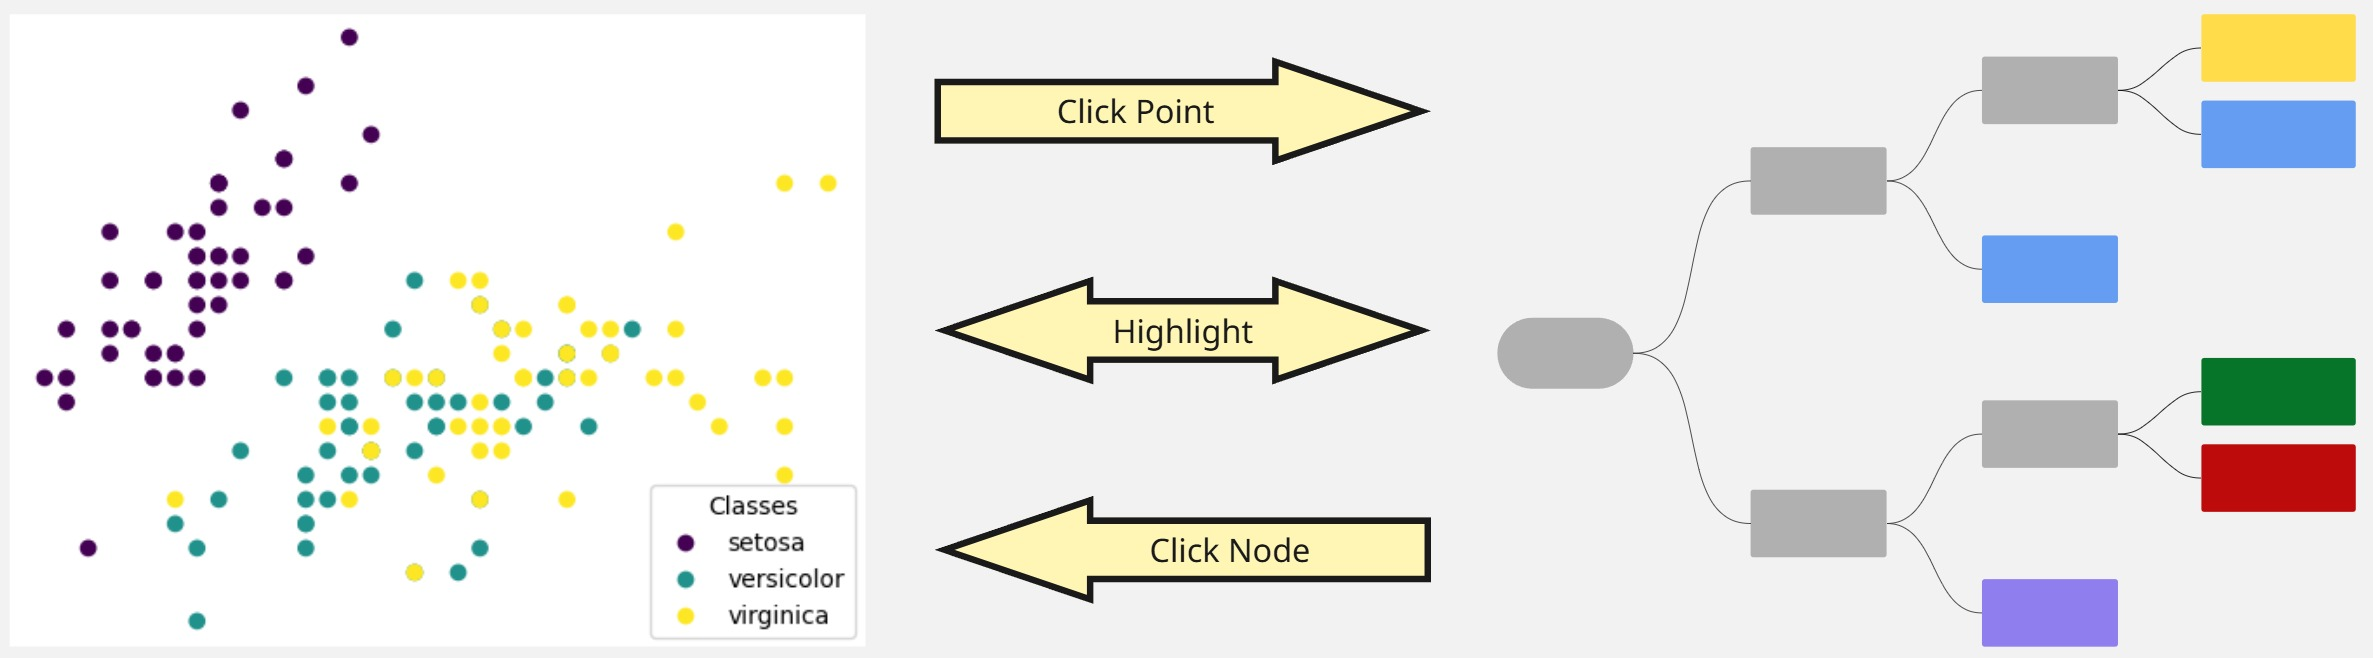
\includegraphics[width=\textwidth]{images/dual_representation_strategy.jpg}
  \caption{Dual representation strategy showing scatter plot visualization of synthetic neighborhood (left), decision tree visualization of rule structure (right), and bidirectional information bridging mechanisms (center arrows)}
  \label{fig:dual_representation_strategy}
\end{figure}

\subsubsection{Configuration Interface Component}

To support the integrated visualization framework, we developed a comprehensive configuration interface that enables users to control all aspects of the $\text{LORE}_{sa}$ explanation generation process. This interface serves as the primary entry point for setting up visualization scenarios and was designed initially for testing purposes, but was later reshaped with the ultimate scope of supporting educational applications.

% \textbf{Dataset and Model Configuration}: 
The interface, when loaded in its demo version, provides structured selection mechanisms for datasets and classification algorithms, enabling users to explore explanations across different domains and model types. This supports the pedagogical goal of demonstrating how explanation quality and characteristics vary across different machine learning contexts.
%
% \textbf{Parameter Management}: 
Comprehensive parameter configuration enables fine-tuning of both the underlying classifier and the $\text{LORE}_{sa}$ explanation generation process. Users can adjust genetic algorithm parameters, and neighborhood generation settings to observe their impact on explanation quality and visualization effectiveness.

% \textbf{Feature Input Interface}: 
Dynamic feature input controls adapt to the selected dataset's characteristics, providing appropriate input mechanisms for numeric, categorical, and ordinal features. This enables users to specify instances for explanation interactively, supporting exploratory analysis workflows where users can investigate how different feature combinations affect both predictions and explanations.
% 
% \textbf{Visualization Control}: 
Additionally, integrated controls for dimensionality reduction technique selection and visualization parameters enable users to compare how different projection methods affect neighborhood visualization quality.

The interface follows established human-computer interaction principles for complex configuration tasks, employing progressive disclosure to manage complexity and providing immediate visual feedback through the coordinated visualization components below.

\subsubsection{Neighborhood 2D Projection Component: Spatial Neighborhood Analysis}

The neighborhood 2D projection serves as the primary interface for understanding the spatial characteristics of the synthetic data. High-dimensional synthetic instances are projected into two-dimensional coordinate systems to enable visual exploration.

Our implementation supports multiple dimensionality reduction techniques to accommodate different analytical requirements, with selection controlled through the configuration interface. \textbf{Uniform Manifold Approximation and Projection (UMAP)} offers nonlinear manifold learning with superior computational efficiency compared to t-SNE \cite{mcinnes2020umapuniformmanifoldapproximation,yang2021dimensionality}, providing intuitive hyperparameter control over local structure preservation and cluster tightness. \textbf{Principal Component Analysis (PCA)} provides a deterministic linear transformation preserving linearity of decision boundaries \cite{sewell2008pca}, enabling direct projection of surrogate model boundaries into the visualization space. 

Color-coded class labeling distinguishes prediction outcomes within synthetic neighborhoods, enabling immediate identification of decision boundary regions and assessment of genetic algorithm instance generation quality.

\subsubsection{Surrogate Model Component: Hierarchical Rule Structure}

The surrogate model component provides hierarchical visualization of logic extracted from 
% $\text{LORE}_{sa}$'s
the
surrogate model, employing \textbf{node-link diagrams} following established best practices \cite{Streeb2021TaskBasedVI}.

\textbf{Node Visual Encoding}: Split nodes (logical conditions and feature thresholds) employ neutral color schemes emphasizing decision point roles, while leaf nodes receive class-specific coloring corresponding directly to spatial neighborhood analysis plot color mapping. \textbf{Edge Visualization} uses variable width encoding to indicate synthetic instance flow through decision branches, with text labels clearly indicating logical conditions and color coding enabling decision path following.

\subsubsection{Bidirectional Information Bridging}

The main interaction mechanisms lie in the \textbf{bidirectional information bridging} that creates explicit connections between spatial and symbolic representations.

% \textbf{Spatial-to-Logical Bridging}: 
User interactions with spatial neighborhood analysis plot points highlight corresponding decision paths in the tree visualization. Clicking synthetic instances traces feature values through the decision tree structure, highlighting complete root-to-leaf classification paths. This enables understanding of how spatial proximity corresponds to logical similarity in decision rules.

% \textbf{Logical-to-Spatial Bridging}: 
On top of that, 
decision tree node interactions highlight corresponding synthetic instances in spatial neighborhood analysis plots. Leaf node clicks highlight all instances satisfying complete logical paths, while split node clicks highlight instances passing through specific decision points, visualizing the spatial distribution of instances satisfying particular logical conditions.

\subsection{Interactive Confirmation Model}

Our interaction model transforms explanation consumption from passive acceptance into active analytical investigation through \textbf{exploratory confirmation} principles. The model begins with comprehensive configuration controls enabling users to establish explanation scenarios, then implements \textbf{details-on-demand} through hover interactions, \textbf{coordinated highlighting} maintaining visual connections, and \textbf{progressive disclosure} enabling incremental exploration.

\subsubsection{Confirmation Systems}

% \textbf{Contextual Tooltip Systems}: 
Sophisticated details-on-demand for both spatial and symbolic elements
are provided through the contextual tooltip systems. 
Spatial neighborhood analysis plot's points tooltips reveal decoded feature values and class prediction information. Decision tree tooltips provide node-specific contextual information, including logical conditions in natural language, sample statistics, and feature importance metrics.

% \textbf{Decision Boundary Visualization}: 
On top of that,
\textbf{Voronoi diagram overlays} provide explicit decision boundary visualization within spatial neighborhood analysis plot space for linear transformations (PCA). Semi-transparent color encoding matching class-based schemes creates colored polygons representing consistent classification areas, enabling assessment of explanation quality through boundary geometric properties and spatial coherence evaluation.